\documentclass[]{article}
\usepackage{lmodern}
\usepackage{amssymb,amsmath}
\usepackage{ifxetex,ifluatex}
\usepackage{fixltx2e} % provides \textsubscript
\ifnum 0\ifxetex 1\fi\ifluatex 1\fi=0 % if pdftex
  \usepackage[T1]{fontenc}
  \usepackage[utf8]{inputenc}
\else % if luatex or xelatex
  \ifxetex
    \usepackage{mathspec}
  \else
    \usepackage{fontspec}
  \fi
  \defaultfontfeatures{Ligatures=TeX,Scale=MatchLowercase}
\fi
% use upquote if available, for straight quotes in verbatim environments
\IfFileExists{upquote.sty}{\usepackage{upquote}}{}
% use microtype if available
\IfFileExists{microtype.sty}{%
\usepackage{microtype}
\UseMicrotypeSet[protrusion]{basicmath} % disable protrusion for tt fonts
}{}
\usepackage[unicode=true]{hyperref}
\hypersetup{
            pdftitle={I/O analysis of climate applications},
            pdfauthor={Arne Beer, MN 6489196, Frank Röder, MN 6526113},
            pdfborder={0 0 0},
            breaklinks=true}
\urlstyle{same}  % don't use monospace font for urls
\usepackage{graphicx,grffile}
\makeatletter
\def\maxwidth{\ifdim\Gin@nat@width>\linewidth\linewidth\else\Gin@nat@width\fi}
\def\maxheight{\ifdim\Gin@nat@height>\textheight\textheight\else\Gin@nat@height\fi}
\makeatother
% Scale images if necessary, so that they will not overflow the page
% margins by default, and it is still possible to overwrite the defaults
% using explicit options in \includegraphics[width, height, ...]{}
\setkeys{Gin}{width=\maxwidth,height=\maxheight,keepaspectratio}
\IfFileExists{parskip.sty}{%
\usepackage{parskip}
}{% else
\setlength{\parindent}{0pt}
\setlength{\parskip}{6pt plus 2pt minus 1pt}
}
\setlength{\emergencystretch}{3em}  % prevent overfull lines
\providecommand{\tightlist}{%
  \setlength{\itemsep}{0pt}\setlength{\parskip}{0pt}}
\setcounter{secnumdepth}{0}
% Redefines (sub)paragraphs to behave more like sections
\ifx\paragraph\undefined\else
\let\oldparagraph\paragraph
\renewcommand{\paragraph}[1]{\oldparagraph{#1}\mbox{}}
\fi
\ifx\subparagraph\undefined\else
\let\oldsubparagraph\subparagraph
\renewcommand{\subparagraph}[1]{\oldsubparagraph{#1}\mbox{}}
\fi

\title{I/O analysis of climate applications}
\author{Arne Beer, MN 6489196, Frank Röder, MN 6526113}
\date{}

\begin{document}
\maketitle

{
\setcounter{tocdepth}{3}
\tableofcontents
}
\pagebreak

\section{Introduction}\label{introduction}

\subsection{About the paper and our
goals}\label{about-the-paper-and-our-goals}

In this paper we analyse and present the pros and cons of different data
structures required by a some carefully picked climate and weather
prediction models. Further we look at the absolute bare minimum of data
required by those models. To consider the pre- and post-processing of
data and the moment where it is really needed at a certain point is also
a very important question to mention. To get an idea about the
importance of data management and processing we had to look at different
kind of models for climate.

In the following sections we will get into some models and show our
progress while setting them up. At the end we will have a talk about the
life-cycle of data.

\subsection{Getting started}\label{getting-started}

With intent to get an overview about the richness of climate,land,ice,
weather and ocean models we took a look at some in depth to work out
that the approachability and documentation was not that clear. Tons of
very old models passed our way of searching through the sides of got
dusty projects and source code. The question than was to get an good
overview of up to date and easy to handle models which are still
supported and updated. For this purpose we put a table together where we
could choose from the best ones which were sounding promising to us. We
came across models with broken scripts and bad documentation, which was
not very obvious on the first glance. So we take a path of trial and
error or giving up, because we faced broken scripts and problem deep
inside the code.

\pagebreak

\section{IFS - Integrated Forecasting
System}\label{ifs---integrated-forecasting-system}

\subsection{About IFS}\label{about-ifs}

IFS has been chosen to be the first model for our research. IFS is a
Model by European Center for Medium-range Weather Forecast (ECMWF) which
is used to make analysis of data. This data can be a variety of
different physical bulks. ECMWF offers a semi open-source version of
their model for research institutions, which is called OpenIFS. The
source code of this model can be obtained by requesting a license for
the institution one is working for. They provide a good documentation
about their model, which cover instruction for building, running
simulations as well as very detailed information about the mathematics
and techniques used in their model. After some research and two weeks
passed we discovered a passage in their license, which forbids
``Commercial and benchmarking use of OpenIFS models''. As our original
research goal is some kind of benchmarking we were forced to stop and
switch to another model. We still recommend to use this model in a
research or academic context, as there is plenty of documentation and a
big user base.

\section{Further progress}\label{further-progress}

After the license incident with IFS we had to look for other open source
models we could use for our research. We looked at many models in the
following we will list some of the most promising: WRF, CFS, GDAS, GFS,
GEFS, CM2.X, GISS GCM ModelE, CESM, MITgcm, GEOSCI, Hector v1.0,
MAGICC/SCENGEN, Metview, COSMO, SAGA, MPI-ESM, ECOHAM

The lookup for new models took about two weeks. Most of the models
mentioned above had serious flaws which forbid us to use them in our
research. Many of them have stopped being maintained many years ago. In
some cases there was no license provided with no available support for
clarifying legal questions. In other cases it was only possible to
obtain a license for our specific research goal by buying it or it was
even completely forbidden to use it for benchmarking purposes, as with
OpenIFS.

Eventually we decided to focus our work on Community Earth System Model
(CESM) and Ecosystem model, Hamburg (ECOHAM). Further we decided to take
a look at AWIPS2 a tool for displaying processed weather forecast and a
very good server for handling data.

\pagebreak

\section{Unidata - Awips2}\label{unidata---awips2}

AWIPS2 is a package which contains weather forecast display and
analysis. This open-source \texttt{Java} application consists of
\texttt{EDEX} a data server and CAVE the client for data analysis and
rendering.

\begin{figure}[htbp]
\centering
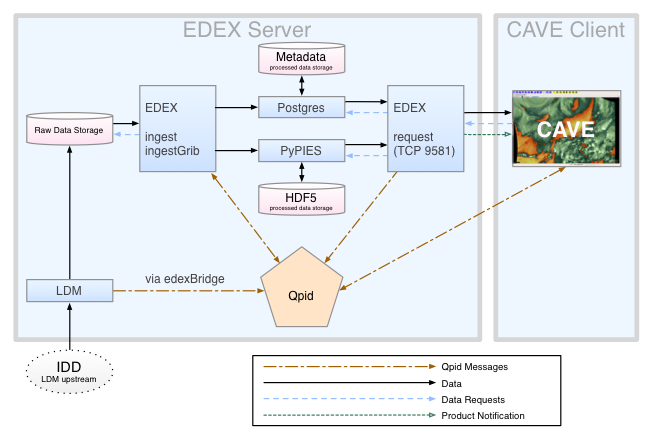
\includegraphics{pics/awips2_coms.png}
\caption{AWIPS2 System}
\end{figure}

\subsection{EDEX (Environmental Data EXchange
)}\label{edex-environmental-data-exchange}

\textbf{EDEX} is the server for AWIPS2 which is used mainly for
preparing the data for CAVE. There are different parts the server is
containing of.

The first source for data is the LDM the Local Data Manager as a piece
of software to share data with computers in other networks. The LDM can
handle different kinds of data from National Weather Service data stream
to radar data, satellit images and grid data from numerical forecast
models. The data could be get directly from the source or a LDM can
communicate with another LDM. When the LDM received data inside the
EDEX, there is a message being send to the \textbf{Qipd} which is the
Apache \textbf{Queue Processor Interface Daemon} spreading the the
availabilty of a data ready for processing. EDEX can decode the data to
make it ready for additional processing or telling CAVE that it is
available for displaying. All of those messages are communicated via
\textbf{edexBridge} The PostgreSQL or Postgres in short is relevant for
the storage and the requests metadata, database tables and already
decoded data. Postgres itself is a relational database management system
which reads and storage the EDEX metadata. The database size is not
limited and it can handle 32 TB of database table capacity.

HDF5 fully spelled Hierarchical Data Format (v.5) is the main format
used in AWIPS2 to store processed grids, images and so on. It is
nowadays very similar to netCDF, which is developed by Unidata. HDF5 can
handle many different types just in one single file.

The \textbf{Python Process Isolated Enhanced Storage} PyPIES created
just for AWIPS2 is used for the writes and reads of data in HDF5 files.
It is very similar to the Postgre but it only processes the requests
related to the HDF5 files. The intention was to isolate the EDEX from
the HDF5 processes.

\subsection{CAVE (Common AWIPS Visualization
Environment)}\label{cave-common-awips-visualization-environment}

\textbf{CAVE} as a part of Awips2 is a tool for data visualisation and
rendering. Its normaly installed on a seperated workstation apart from
the other AWIPS2 parts.

\begin{figure}[htbp]
\centering
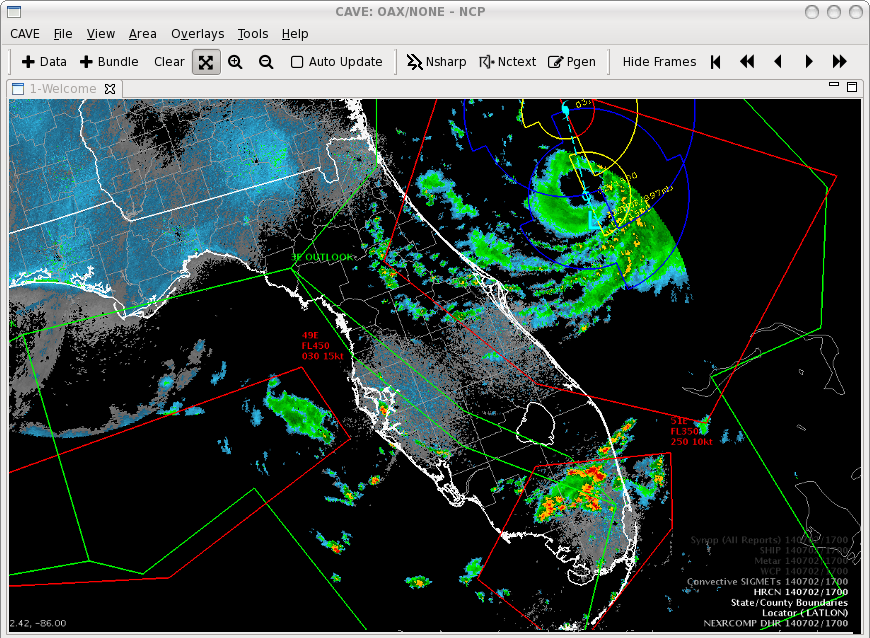
\includegraphics{pics/Unidata_AWIPS2_CAVE.png}
\caption{CAVE Example}
\end{figure}

\subsection{Installation}\label{installation}

For the installation of \texttt{Awips2} you can easily download the
repository from Github and make it run with \texttt{installCave.sh} and
\texttt{installEDEX.sh}. Those install scripts use yum as a package
manager are currently supported for CentOS, Fedora and RedHead. To make
it compatible for the cluster there is maybe more to be done. Awips2 is
normally installed with the help of the package manager YUM which could
lead to some problems if you' re not the root. Awips2 requires a
directory at root location ``/awips2/''. There are about 2000 lines of
code where ``/awips2/'' is hard-coded, so switching directories is not
an option.

\textbf{To build} a version for our purpose it would be the best to have
a EDEX on the cluster which is providing our local CAVE with data for
visualization.

\pagebreak

\section{CESM - Community Earth System
Model}\label{cesm---community-earth-system-model}

\subsection{About CESM}\label{about-cesm}

CESM itself consists of seven geophysical models like ocean, land, ice,
atmosphere \ldots{} . The CESM project is made and supported by U.S.
climate researchers and mainly by the National Science Foundation (NSF).
If there are different models in use, a so called coupler handle the
time progression and overall management between coupled systems through
sequences of communication. The scientific development is conducted by
the CESM working group twice a year. For more information related to the
development its recommended to visit the website {[}link to source{]}.
Additional CESM can be most of the time run out-of-the-box the
developers claiming. ``Bit-for-bit reproducibility'' cannot be
guarnteed, because of using different compilers and system versions.

\subsection{Requirements}\label{requirements}

Here are some preconditions directly taken from the documentation of
CESM. In favour to make it run on the cluster we are working with we
have to walk through the list:

\begin{itemize}
\tightlist
\item
  UNIX style operating system such as CNL, AIX and Linux \checkmark
\item
  csh, sh, and perl scripting languages \checkmark
\item
  subversion client version 1.4.2 or greater \checkmark
\item
  Fortran (2003 recommended, 90 required) and C compilers. pgi, intel,
  and xlf are recommended compilers. \checkmark (gfortran gcc-Version
  4.8)
\item
  MPI (although CESM does not absolutely require it for running on one
  processor) \checkmark
\item
  NetCDF 4.2.0 or newer. \checkmark (Version 7.3 \& 4.2)
\item
  ESMF 5.2.0 or newer (optional).
\item
  pnetcdf 1.2.0 is required and 1.3.1 is recommended (optional)
\item
  Trilinos may be required for certain configurations X
\item
  LAPACKm or a vendor supplied equivalent may also be required for some
  configurations. \checkmark (Version 3.0)
\item
  CMake 2.8.6 or newer is required for configurations that include CISM.
  \checkmark (Version 2.8.12.2)
\end{itemize}

\subsection{Installation}\label{installation-1}

\begin{itemize}
\item
  Open source
\item
  Download at
  \href{http://www.cesm.ucar.edu/models/cesm1.2/cesm/doc/usersguide/x290.html\#download_ccsm_code}{CCMS(Link)}:

  \begin{itemize}
  \tightlist
  \item
    Username: guestuser
  \item
    Password: friendly
  \end{itemize}
\item
  Version 1.2.1
\item
  Available with svn:

\begin{verbatim}
svn co https://svn-ccsm-models.cgd.ucar.edu/cesm1/release_tags/cesm1_2_1 \
cesm1_2_1 --username guestuser --password friendly
\end{verbatim}
\item
  We recommend to create an entry in your
  \texttt{\textasciitilde{}/.subversion/servers} config for later svn
  usage with scripts:

\begin{verbatim}
[groups]
cesm = svn-ccsm-inputdata.cgd.ucar.edu

[cesm]
username = guestuser
store-passwords = yes
\end{verbatim}
\end{itemize}

Most parts of the CESM software project are open source. However three
libraries are published by the Los Almos National Laboratory, who
licensed their software as free to use as long as it isn't used in a
commercial context. Affected libraries are POP, SCRI and CICE
\href{http://www.cesm.ucar.edu/management/UofCAcopyright.ccsm3.html}{(Link
to licence)}.

\subsection{Input Data Set}\label{input-data-set}

\subsubsection{Setup}\label{setup}

There is actually a set of input data which can be downloaded and
configured for CESM. It can be made available through another Subversion
input data repository by using the same user name as used in the
installation above. The dataset is around 1 TB big and should not be
downloaded at ones. The download is regulated on demand, so if CESM
needs the particular data it will be downloaded and checked
automatically be CESM itself. The data should be on a disk in the local
area. The CESM variable \texttt{\$DIN\_LOCK\_ROOT} has to be set inside
of the script. Multiple users can use the same
\texttt{\$DIN\_LOCK\_ROOT} directory and should be configured as group
writable. If the machine is supported there is a preset otherwise there
is a possibility to make it also run on generic machines with the
variable as argument for the \texttt{./scripts/create\_newcase} script .
Files in the subdirectory of the \texttt{\$DIN\_LOCK\_ROOT} should be
write-protected to exclude accidentally deleting or changing of them. As
we are executing our CESM executable there is the utility
\texttt{check\_input\_data} which is called to locate all the needed
input data for a certain case. When this data is not found in
\texttt{\$DIN\_LOCK\_ROOT} it will automatically be downloaded by the
scripts or the user using the \texttt{check\_input\_data} with -export
as command argument. If ones like to download the input manually it
should be done \textbf{before} building CESM. In addition it is also
possible to download the data via svn subcommands direct, but it is much
better to use the \texttt{check\_input\_data} script as it secures to
download only the required data.

\subsection{CESM Creating And Configure A New
Case}\label{cesm-creating-and-configure-a-new-case}

As we are executing our CESM executable there is the utility
\texttt{check\_input\_data} which is called to locate all the needed
input data for a certain case. When this data is not found in
\texttt{\$DIN\_LOCK\_ROOT} it will automatically be downloaded by the
scripts or the user using the \texttt{check\_input\_data} with -export
as command argument. If ones like to download the input manually it
should be done \textbf{before} building CESM. In addition it is also
possible to download the data via SVN subcommands direct, but it is much
better to use the \texttt{check\_input\_data} script as it secure to
download only the required data.

\subsubsection{Prerequisites}\label{prerequisites}

We need the \texttt{perl-switch} for the project setup.

\subsubsection{Create a new case}\label{create-a-new-case}

Cases are pretty much a thing. But we don't know what they are\ldots{}
To create a case execute \texttt{./scripts/create\_newcase} with correct
parameters, e.g.:

\begin{verbatim}
    # Parameters are respectively:
    # Case name and directory location
    # Machine name
    # Component set name
    # Resolution
    /create_newcase -case ./test1 \
        -mach userdefined \
        -compset B1850CN  \
        -res f45_g37
\end{verbatim}

In the original repository many errors occur due to deprecated syntax
and buggy setup code. We recommend to use our updated version of the
code. The text \texttt{Successfully\ created\ the\ case} should appear
on your screen. Will the problem with \texttt{create\_newcase}remain,
once should try one of the examples listed in the error message.

In case \texttt{create\_newcase} breaks while calling one of the
\texttt{mkbatch.*} scripts, you probably need to install CShell, as
those scripts are written for \texttt{\#!/bin/csh}.

The result of \texttt{create\_newcase} is a directory
\texttt{.../cesm/scripts/\textless{}YourCase\textgreater{}} with a bunch
of directorys or filenames to be explained:

\begin{verbatim}
README.case - This files will contain tracked problems and changes at runtime
CaseStatus  - A File containing a history of operations done in the actual case
BuildConf/  - A never have to be edit directory with scripts for generating component namelists and utility libraries
SourceMods/ - This directory is for modified source code
LockedFiles/    - It contains copies of files that should not be changed, xml are locked until the clean operation is executed
Tools/      - A never have to be edit location with support scripts
env_mach_specific   - machine-specific variables for building/running are set here
env_case.xml    - Case specific variables like the root and models are set(cannot be changed, have to re-run create_newcase for changes)
env_build.xml   - contains the building settings, resolution and configuration options
env_mach_pers.xml   - sets the machine processor layout
env_run.xml - contains run-time settings
cesm_setup  - script for set up
$CASE.$MACH.build   - script for building components, executables and utility libraries
$CASE.$MACH.clean_build - remove all object files and libraries
$CASE.$MACH.l_archive   - script for long-term archiving of output (only if it is available on the machine)
xmlchange   - utility to change values in other .xml files
preview_namelists   - utility to see the component namelists
check_input_data    - check for input datasets
check_production_test   - creates a test of the owners case
\end{verbatim}

\subsubsection{Setup case}\label{setup-case}

Once a case has been created by the previous command, the setup for case
has to be completed. To achieve this, the \texttt{cesm\_setup} script in
the case directory needs to be executed. Settings for this specific case
are specified in \texttt{env\_mach\_pes.xml}. The documentation states
that this file should only be manipulated using \texttt{xmlchange}. As
we want to use our own machine, we need to create a user defined machine
for this test case.

Values that need to be set:

\begin{itemize}
\tightlist
\item
  \texttt{MAX\_TASKS\_PER\_NODE} in \texttt{env\_mach\_pes.xml}
\item
  \texttt{OS} in \texttt{env\_build.xml}
\item
  \texttt{MPILIB} in \texttt{env\_build.xml}
\item
  \texttt{COMPILER} in \texttt{env\_build.xml}
\item
  \texttt{EXEROOT} in \texttt{env\_build.xml}
\item
  \texttt{RUNDIR} in \texttt{env\_run.xml}
\item
  \texttt{DIN\_LOC\_ROOT} in \texttt{env\_run.xml}
\end{itemize}

There is an example configuration in \texttt{scripts/example\_config}.
This configuration expects a folder in root \texttt{/cesm} and
\texttt{/cesm/inputdata}, but if you don't have root access at your
location, those variables can be easily changed (\texttt{EXEROOT},
\texttt{RUNDIR}, \texttt{DIN\_LOC\_ROOT})

\subsubsection{Build case}\label{build-case}

To build a case, the \texttt{\$CASENAME.build} script needs to be
executed. In case you chose the \texttt{gnu} compiler in your settings,
make sure you have \texttt{gmake} installed and create a symlink
\texttt{gmake} to \texttt{make}. If any previous builds failed,
\texttt{\$CASENAME.clean\_build} has to be executed.

\subsubsection{Getting data}\label{getting-data}

The data download script lies directly in
\texttt{cesm1\_2\_1/scripts/"yourcase"} you created one step back. To
download input data to a specific data directory execute this, with an
adjusted path.

\begin{verbatim}
     export DIN_LOC_ROOT='/Path/to/input/data/dir'
     mkdir -p $DIN_LOC_ROOT
    ./check_input_data -inputdata $DIN_LOC_ROOT -export -datalistdir $DIN_LOC_ROOT  
\end{verbatim}

Now it also should be possible to check if the requiered data is present
with follow command:

\begin{verbatim}
check_input_data -inputdata $DIN_LOC_ROOT -check
\end{verbatim}

To download missing data from the server use:

\begin{verbatim}
check_input_data -inputdata $DIN_LOC_ROOT -export
\end{verbatim}

Booth commands need to be run inside the \texttt{\$CASEROOT}

\subsubsection{Build the Case}\label{build-the-case}

\begin{verbatim}
  cd ~/cesm/EXAMPLE_CASE
  ./cesm_setup
  ./EXAMPLE_CASE.build
\end{verbatim}

\subsection{Quickstart}\label{quickstart}

This Quickstart should give an overview about the work flow of CESM
especially when there is already a version ported to the local target
machine. If there is nothing already ported on the start machine, start
with the more detailed description above.

There are a couple of definitions which must be unterstand and lead you
through this section

\begin{verbatim}
    $COMPSET refers to the components set
    $RES refers to the model resolution
    $MACH refers to the target machine
    $CCSMROOT refers to the CESM root directory
    $CASE refers to the case name
    $CASEROOT refers to the full pathname of the root directory where the case ($CASE) will be created
    $EXEROOT refers to the executable directory ($EXEROOT is normally __not__ the same as $CASEROOT)
    $RUNDIR refers to the directory where CESM actually runs. This is normally set to $EXEROOT/run. (changing $EXEROOT does not change $RUNDIR as these are independent variavles)
\end{verbatim}

As first step you need to
\href{http://www.cesm.ucar.edu/models/cesm1.2/cesm/doc/usersguide/x290.html}{download(Link)}
CESM and select a machine, a component set and a resolution form the
list displayed after using this commands:

\begin{verbatim}
    > cd $CCSMROOT/scripts
    > create_newcase -list
\end{verbatim}

There is a list CESM supported components like
\href{http://www.cesm.ucar.edu/models/cesm1.2/cesm/doc/modelnl/compsets.html}{sets(Link)},
\href{http://www.cesm.ucar.edu/models/cesm1.2/cesm/doc/modelnl/grid.html}{resolution(Link)}
and
\href{http://www.cesm.ucar.edu/models/cesm1.2/cesm/doc/modelnl/machines.html}{machines(Link)}.
Remember, that the \texttt{-list} will always provide a list of
supported component sets for the local CESM version. The first letters
of the \texttt{-compset} option will indicate which kind of model is
used. To create a case the command \texttt{create\_newcase} is used. It
creates a case directory containing the scripts and XML files to set up
the configurations for resolution, component set and machine requested.
The \texttt{create\_newcase} has some arguments as condition and some
additional options for generic machines. For more information
\texttt{create\_newcase\ -h} should help. I case that a supported
machine is in use \texttt{(\$MACH)} tipe the following words:

\begin{verbatim}
    >create_newcase -case $CASEROOT \
            -mach $MACH \
            -compset $COMPSET \
            -res $RES
\end{verbatim}

When using the machine setting \texttt{userdefined} it is requiered to
edit the resulting xml files and fill them with the informations needed
for the target machine. The \texttt{create\_newcase\ -list} command will
also show all available machines for the local version. For running a
new target machine use the \textbf{section below}.

To setup the case run script be sure to use the \texttt{cesm\_setup}
command which creates a \(CASEROOT/\)CASE.run script with
\texttt{user\_nl\_xxx} files, while the xxx tell us something about the
case configuration. But before running \texttt{cesm\_setup} there is the
\texttt{env\_mach\_pes.xml} file in \$CASEROOT to be modified fitting to
the experiment to be run.

\begin{verbatim}
    > cd $CASEROOT
\end{verbatim}

After this the \texttt{env\_mach\_pes.xml} can be modified with the
\textbf{\emph{xmlchange}} command. Take a look at \texttt{xmlchange\ -h}
for detailed information. Then the \texttt{cesm\_setup} can be
initiated.

\begin{verbatim}
    > ./cesm_setup
\end{verbatim}

With the optional build modifications in mind
(\texttt{env\_mach\_pes.xml}) the build script can be startet:

\begin{verbatim}
    > $CASE.build
\end{verbatim}

To run the case and maybe setting the variable \$DOUT\_S in
\texttt{env\_mach\_pes.xml} to \texttt{false} the job can be submitted
to the batch queue:

\begin{verbatim}
    > $CASE.submit
\end{verbatim}

After the job finished you can review all the following directories and
files like:

\begin{verbatim}
    1. $RUNDIR
      * the directory set in the `env_build.xml` file
      * the location where the CESM was run with log files for every part
    2. $CASEROOT/logs
      * if the run was successful the log files have been copied into this directory
    3. $CASEROOT
      * here should a standard out or error file
    4. CASEROOT/CaseDocs
      * a list a case names is copied to this directory
    5. CASEROOT/timing
      * here are timing files which are representing the performance of the model
    6. $DOUTS_S_ROOT/$CASE
      * This directory is an archive depending on the setting done above, while it is true there is a log and history
\end{verbatim}

\subsection{Conclusion}\label{conclusion}

We managed to fix the build scripts to create and setup a case. In the
step of compiling the code we encountered a few errors, but we were able
to compile two models. After that another error occurred during
compilation of the \texttt{pio} module. CESM ships with a parallel IO
library, which practically is a set of interfaces for netcdf, parallel
netcdf or binary IO. We chose to use pnetcdf for our build. After
installing the required libraries and setting the proper paths and
variables as described in their documentation the build still failed and
required a configuration file for \texttt{pio}. There is no further
information about this configuration file in their documentation. After
writing their support without response, we were forced to stop using
CESM.

After all CESM still looks like a promising model, but it has many
flaws. Their build scripts aren't generic. Nearly 3 weeks were spent to
understand the code and fix old syntax or hard-coded paths. If there
were better documentation about the setup and compilation for CESM we
could've probably used it, as we were really close to compiling it.

\section{ECOHAM5}\label{ecoham5}

\subsection{About}\label{about}

ECHAM is a model for atmospheric circulation, which was developed by the
Max Planck Institute for Meteorology. It's a important part of the
MPI-ESM which is the Earth system model of the Max Planck Institute.
ECHAM itself is branched in year 1987 from the global numerical weather
prediction model by ECMWF. Ever scince its developed by Max Planck
Institute.

\subsection{Getting Started}\label{getting-started-1}

\subsubsection{Source Code}\label{source-code}

The \href{http://www.mpimet.mpg.de/en/science/models/license/}{Code for
ECHAM6} might be available here.

\subsubsection{Compile ECOHAM}\label{compile-ecoham}

To compile ECOHAM for a testcase, there is the following script to be
run in different ways:

\begin{verbatim}
./CompileJob-cluster.sh TEST 0  // for just the compiling
./CompileJob-cluster.sh TEST 1  // for compiling and make it ready to run
./CompileJob-cluster.sh TEST 2  // compiling and run the model
\end{verbatim}

In our case \texttt{TEST} is the data input. If an error occures and you
don't have the permission to run \texttt{sbatch} on a specified
partiotions, it is nessecarry to make modification in the
\texttt{RunJob.TEST} located in the folder of the declared input. The
wrk directory will contain the models ouput. The directory
\texttt{Input} inside the wrk folder contain all the input used for the
model run. There are \texttt{.dat} \texttt{.header}and \texttt{.direct}
files which are providing the application with all data needed.

\section{Lifecycle of data}\label{lifecycle-of-data}

\subsection{General}\label{general}

Through the whole process of running a simulation there a different type
of data at certain points. The complexity and the information can
differ. The data which is fed into the program at the beginning won't be
the same which is visualized by a color on the climate overview

The Lifecycle could be divided into those parts:

\begin{enumerate}
\def\labelenumi{\arabic{enumi}.}
\tightlist
\item
  creating data
\item
  processing data (pre- and post-processing included)
\item
  analyzing data
\item
  preserving data
\item
  giving access to data
\item
  re-using data
\end{enumerate}

\subsubsection{Creating the data}\label{creating-the-data}

Creating the data could also be named as design of the research because
it will limit and lead the handling of the application. Which kind of
data management, formats and storage used is another question to be
answered. If there are already similar simulations, data can be found
there for re-use. For not already exsisting simulation the data must be
collected through experiments, measures and also simulations generation
data. Metadata will also be captured and maybe created.

\subsubsection{Processing data}\label{processing-data}

This step will contain the digitization, transcribing and translation of
data into a useful figure. It also is about the vetting of validate and
clean data. To anonymize data needed could also be part of processing.
Sometimes there is pre- and post-proscessing apart from the general
processing. Pre-processing will prepare the particullar data just before
a certain step. It will dimiss all the not needed information to save
time and storage capacity. After such a step there could be another
process called post-processing which is about the treatment of data to
make it useable for other steps afterwards. To make it easy to read for
other people, the data should be described and explained. As the last
step it is nescessary to take a look at the storing of data.

\subsubsection{Analyzing of data}\label{analyzing-of-data}

Because data itself is not very enlightening, especially when there are
thousands of values we need methods to interpret them. Derivation of
data while calculating the output of the research and making
publications is another part. Now that the made our main calculations
with the data we have to prepare it for preservation.

\subsubsection{Preserving of data}\label{preserving-of-data}

Preserving of data is about checking out the best formats and best
mediums on which we backup and store the data. Also creation of metadata
and documentation is important for the final archiving.

\subsubsection{Giving access to data}\label{giving-access-to-data}

Because reseach is done mostly by public institutes there is a demand
for sharing and distribute the data and knowledge. To consider about the
access control and copyrights might also be very useful.

\subsubsection{Re-using data}\label{re-using-data}

Researches in the future could also be based on the work which was done
in the past. Teaching and publications may be good examples for
re-using.

\subsection{Summary}\label{summary}

With the growth of data in simulations and the improvement of processing
power which is much higher than the performace of store power it is very
essential for research establishments. The data and knowledge are the
key and the only thing those institutes are working for. Therefore data
and knowledge needs the right treatment.

\section{Conclusion}\label{conclusion-1}

This project was about the analysis of input and output of climate
applications. We made our way through run models providided by our
supervisors and some we found in the internet which seemed suiteable for
our purpose. We faced bad documentations and insufficient scripts for
making such a model run. At the end we did not get along with most of
them at different levels progress. ECHAM was the only one which worked
on the fly, because of the test which is very well prepared. Apart of
that it didn't keept us away from analysing the life-cycle of data in
general and make a little summary about that.

EDEX \& CAVE are supported by the U.S. company Raytheon.

\section{References}\label{references}

https://www.unidata.ucar.edu/software/ldm/ldm-current/factsheet.html

http://www.cesm.ucar.edu/models/current.html http://www2.cesm.ucar.edu/
http://www.ecmwf.int/en/forecasts/
http://www.unidata.ucar.edu/software/awips2/
https://www.bu.edu/datamanagement/background/data-life-cycle/ Data
Lifecycle

\end{document}
